\documentclass{beamer}
\usetheme{metropolis}

\usepackage{graphicx}
\usepackage{appendixnumberbeamer}

\title{Csoportos döntéshozatal}
\author{Patka Zsolt-András}
\institute{Sapientia EMTE}
\date{2020.03.09}

\begin{document}

\begin{frame}
    \titlepage
\end{frame}

\begin{frame}
\frametitle{Miről lesz szó?}
\tableofcontents
\end{frame}

\section{Bevezető}

\subsection{Sajátosságok}
\begin{frame}{\secname : \subsecname}
    \begin{itemize}
        \item nem egy ember hozza meg a döntést, hanem egy csoport
        \item komplexebb döntések esetén használják
        \item munkahelyi vezetés alsóbb szintjein - egyéni döntések
        \item munkahelyi vezetés felsőbb szintjein - csoportos döntések
    \end{itemize}
\end{frame}

\subsection{Előnyök}
\begin{frame}{\secname : \subsecname}
    \begin{itemize}
        \item több ismeret, információ
        \item többféle probléma-megközelítés kerül felszínre
        \item a csoport teljesítménye gyakran jobb, mint az átlagos csoporttagé
        \item a döntés elfogadtatása sokkal könnyebb
    \end{itemize}
\end{frame}

\subsection{Hátrányok}
\begin{frame}{\secname : \subsecname}
    \begin{itemize}
        \item hosszabb időt vesz igénybe
        \item előfordulhat, hogy egyetlen személy uralja a folyamatot
        \item rossz megoldás elfogadása, beletörődés
        \item csoportnyomás
    \end{itemize}
\end{frame}


\section{Módszerek}

\subsection{Brainstorming}
\begin{frame}{\secname : \subsecname}

A brainstorming (ötletbörze) lényege az, hogy a gondolkodási folyamat ne legyen megszakítva.

Moderátor: \textbf{ajánlott}

Szabályai:
\begin{enumerate}
    \item fókuszálj a mennyiségre
    \item ne kritizálj
    \item osszd meg az ötleteidet, még akkor is ha ezek szokatlanok
    \item kombináld és javítsd az ötleteket
\end{enumerate}

Menete:
\begin{enumerate}
    \item valaki bemutatja a problémát
    \item a csoport elkezd ötletelni, az ötleteket leírják egy táblára
    \item a végén kiértékelik az ötleteket
\end{enumerate}
\end{frame}

\subsection{6-3-5-ös módszer}
\begin{frame}{\secname : \subsecname}

6 fős csoport 3 gondolatot 5-ször továbbfejleszt.

Moderátor: \textbf{nélkülözhető}

Menete:
\begin{enumerate}
    \item mindenki kap egy lapot egy 6x3-as táblázattal
    \item 5 perc alatt mindenki leír 3 ötletet a táblázatba
    \item mindenki továbbadja a lapot a nála balra ülőnek
    \item 5 perc alatt mindenki a már leírt 3 ötletet továbbviszi egy-egy újabb ötlettel
    \item a 6 kör lejárta után minden résztvevő minden lapon bejelöli azt a 3 ötletet ami neki a legjobban tetszik
    \item a legnépszerűbb ötleteket felírják egy táblára és tovább tárgyalják
\end{enumerate}

\end{frame}

\subsubsection*{Példa (1/6)}
\begin{frame}{\subsecname : \subsubsecname}
    \begin{table}[H]
	\begin{center}
		\caption{Csokoládépudding - 635 módszer}
		\begin{tabular}{l|c|c|c}
		\textbf{Anna}   & új csomagolás 	                                                                & hűségpontok                                                           & kevesebb cukor \\
		\hline         
        \textbf{Gábor}  &  	& & \\
        \hline         
        \textbf{Attila} &   & & \\
        \hline         
        \textbf{László} &   & & \\
        \hline         
        \textbf{Kinga}  &   & & \\
        \hline         
        \textbf{Noémi}  &   & & \\
		\end{tabular}
	\end{center}
\end{table}
\end{frame}

\subsubsection*{Példa (2/6)}
\begin{frame}{\subsecname : \subsubsecname}
    \begin{table}[H]
	\begin{center}
        \caption{Csokoládépudding - 635 módszer}
        \scalebox{0.7}{
		\begin{tabular}{p{1.5cm}|p{4cm}|p{4cm}|p{4cm}}
		\textbf{Anna}   & új csomagolás 	                                                                & hűségpontok                                                           & kevesebb cukor \\
		\hline         
        \textbf{Gábor}  & bombon formájában 	                                                            & hűségkártya                                                           & hangsúlyozni az egészséges étkezést \\
        \hline         
        \textbf{Attila} & & & \\
        \hline         
        \textbf{László} & & & \\
        \hline         
        \textbf{Kinga}  & & & \\
        \hline         
        \textbf{Noémi}  & & & \\
        \end{tabular}
        }
	\end{center}
\end{table}
\end{frame}

\subsubsection*{Példa (3/6)}
\begin{frame}{\subsecname : \subsubsecname}
    \begin{table}[H]
	\begin{center}
        \caption{Csokoládépudding - 635 módszer}
        \scalebox{0.7}{
		\begin{tabular}{p{1.5cm}|p{4cm}|p{4cm}|p{4cm}}
		\textbf{Anna}   & új csomagolás 	                                                                & hűségpontok                                                           & kevesebb cukor \\
		\hline         
        \textbf{Gábor}  & bombon formájában 	                                                            & hűségkártya                                                           & hangsúlyozni az egészséges étkezést \\
        \hline         
        \textbf{Attila} & pudding bombonban       	                                                        & hűségpontok és hűségkártya az egész pudding termékvonalra             & az egészség jólléthez vezet, a csokoládé boldoggá tesz \\
        \hline         
        \textbf{László} & & & \\
        \hline         
        \textbf{Kinga}  & & & \\
        \hline         
        \textbf{Noémi}  & & & \\
        \end{tabular}
        }
	\end{center}
\end{table}
\end{frame}

\subsubsection*{Példa (4/6)}
\begin{frame}{\subsecname : \subsubsecname}
    \begin{table}[H]
	\begin{center}
        \caption{Csokoládépudding - 6-3-5-ös módszer}
        \scalebox{0.7}{
		\begin{tabular}{p{1.5cm}|p{4cm}|p{4cm}|p{4cm}}
		\textbf{Anna}   & új csomagolás 	                                                                & hűségpontok                                                           & kevesebb cukor \\
		\hline         
        \textbf{Gábor}  & bombon formájában 	                                                            & hűségkártya                                                           & hangsúlyozni az egészséges étkezést \\
        \hline         
        \textbf{Attila} & pudding bombonban       	                                                        & hűségpontok és hűségkártya az egész pudding termékvonalra             & az egészség jólléthez vezet, a csokoládé boldoggá tesz \\
        \hline         
        \textbf{László} & a cukorkákat nem kell hűvösen tartani $\rightarrow$ el lehet adni a terméket a kasszánál is  & díjak ha egy bizonyos pontmennyiség el van érve                         & figyelemfelhívó kampányok arról, hogy a csokoládé milyen egészséges \\
        \hline         
        \textbf{Kinga}  & & & \\
        \hline         
        \textbf{Noémi}  & & & \\
        \end{tabular}
        }
	\end{center}
\end{table}
\end{frame}

\subsubsection*{Példa (5/6)}
\begin{frame}{\subsecname : \subsubsecname}
    \begin{table}[H]
	\begin{center}
        \caption{Csokoládépudding - 635 módszer}
        \scalebox{0.7}{
		\begin{tabular}{p{1.5cm}|p{4cm}|p{4cm}|p{4cm}}
		\textbf{Anna}   & új csomagolás 	                                                                & hűségpontok                                                           & kevesebb cukor \\
		\hline         
        \textbf{Gábor}  & bombon formájában 	                                                            & hűségkártya                                                           & hangsúlyozni az egészséges étkezést \\
        \hline         
        \textbf{Attila} & pudding bombonban       	                                                        & hűségpontok és hűségkártya az egész pudding termékvonalra             & az egészség jólléthez vezet, a csokoládé boldoggá tesz \\
        \hline         
        \textbf{László} & a cukorkákat nem kell hűvösen tartani -> el lehet adni a terméket a kasszánál is  & díjak ha egy bizonyos pontmennyiség el van érve                         & figyelemfelhívó kampányok arról, hogy a csokoládé milyen egészséges \\
        \hline         
        \textbf{Kinga}  & gyűjtőalbumot lehetne adni a kasszánál a gyerekeknek       	                    & a pontokat be lehet váltani matricákra                                & kiegyensúlyozott, boldog és egészséges család a csokoládépudding fogyasztása által \\
        \hline         
        \textbf{Noémi}  & & & \\
        \end{tabular}
        }
	\end{center}
\end{table}
\end{frame}

\subsubsection*{Példa (6/6)}
\begin{frame}{\subsecname : \subsubsecname}
    \begin{table}[H]
	\begin{center}
        \caption{Csokoládépudding - 6-3-5-ös módszer}
        \scalebox{0.7}{
		\begin{tabular}{p{1.5cm}|p{5cm}|p{4cm}|p{4cm}}
		\textbf{Anna}   & új csomagolás 	                                                                & hűségpontok                                                           & kevesebb cukor \\
		\hline         
        \textbf{Gábor}  & bombon formájában 	                                                            & hűségkártya                                                           & hangsúlyozni az egészséges étkezést \\
        \hline         
        \textbf{Attila} & pudding bombonban       	                                                        & hűségpontok és hűségkártya az egész pudding termékvonalra             & az egészség jólléthez vezet, a csokoládé boldoggá tesz \\
        \hline         
        \textbf{László} & a cukorkákat nem kell hűvösen tartani $\rightarrow$ el lehet adni a terméket a kasszánál is  & díjak ha egy bizonyos pontmennyiség el van érve                         & figyelemfelhívó kampányok arról, hogy a csokoládé milyen egészséges \\
        \hline         
        \textbf{Kinga}  & gyűjtőalbumot lehetne adni a kasszánál a gyerekeknek       	                    & a pontokat be lehet váltani matricákra                                & kiegyensúlyozott, boldog és egészséges család a csokoládépudding fogyasztása által \\
        \hline         
        \textbf{Noémi}  & kitöltött gyűjtőalbumot be lehet cserélni egy ingyenes belépőre az állatkertbe    & az első 5 aki 1000 pontot összegyűjt, meg lesz hívva a puddinggyárba  & családi kirándulásokat finanszírozni \\
        \end{tabular}
        }
	\end{center}
\end{table}
\end{frame}

\subsection{Philips 66-os módszer}
\begin{frame}{\secname : \subsecname}
6 fős csoport 6 perces megbeszélés alatt próbál megoldani egy problémát.

Moderátor: \textbf{szükséges}

Menete:
\begin{enumerate}
    \item a résztvevőket csoportra osszák
    \item mindegyik csoport külön tart egy ötletbörzét
    \item az idő lejárta után minden csoport kiválasztja a legjobb ötleteit és ezt bemutatja mindenki előtt
\end{enumerate}
\end{frame}

\subsection{Edward de Bono 6 gondolkodó kalap}
\begin{frame}{\secname : \subsecname}
\begin{columns}
\column{0.2\textwidth}
\centering
Moderátor: \textbf{szükséges} \\
\vspace{5mm}
6 kalap 6 gondolkodási módot képvisel
\column{0.8\textwidth}
\centering
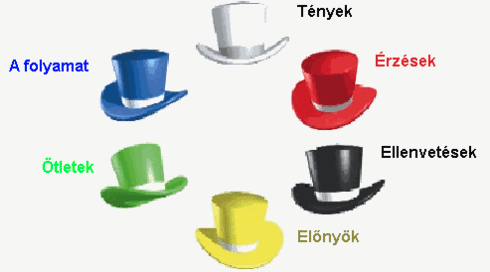
\includegraphics[scale=0.4]{figures/hatkalap.png}

\begin{footnotesize}
forrás: \url{https://hu.wikipedia.org/wiki/Hat_gondolkod\%C3\%B3_kalap}
\end{footnotesize}
\end{columns}
\end{frame}

\section{Esettanulmány - HP és Compaq}
\begin{frame}
\textbf{Probléma:} 2002 májusi Hewlett-Packard és Compaq egyesülése

\textbf{Megoldás:}
\begin{itemize}
    \item Előzmények:
    \begin{itemize}
        \item minden csapattag tényeket, információt és részleteket kellett gyűjtsön a terveiről
    \end{itemize}
    \item Meetingsorozat napja:
    \begin{enumerate}
        \item fehér kalap - hiányzó információ begyűjtése
        \item sárga kalap - előnyök
        \item fekete kalap - veszélyek, kihívások
        \item zöld kalap - megoldások
        \item zöld kalap - laterális gondolkodás
        \item piros kalap - megérzések
        \item kék kalap - összegzés
    \end{enumerate}
    \item a bemutatók kb. 25 percet tartottak
\end{itemize}

\end{frame}


\begin{frame}
\centering
{\Huge Köszönöm a figyelmet!}
\end{frame}

\appendix{Források}
\begin{footnotesize}
    \begin{itemize}
        \item Döntéselmélet, Szikora Péter, Óbudai Egyetem - Döntéselmélet – 2016
        \item \url{http://centroszet.hu/tananyag/vezetes/442_csoportos_dnts.html}
        \item \url{http://leewardteam.com/wp-content/uploads/2017/09/case-study-hp.pdf}
        \item \url{https://penzugysziget.hu/}
        \item InnovationNet: The art of creating and benefiting from innovation networks, Jan Kratzer
        \item \url{https://axel-schroeder.de/}
        \item \url{https://de.wikipedia.org/wiki/Discussion_66}
        \item \url{http://comscientia.com/training_course_examples/ctl/pages/Phillips\%2066\%20(buzz\%20sessions).pdf}
        \item \url{http://www.debonogroup.com/six_thinking_hats.php}
    \end{itemize}
\end{footnotesize}

\end{document}